

\actTitle{Worksheet 3.2-3.4 Review}

\noindent \textbf{Instructions:}  Work together in groups of  3 or 4 to complete the following problems.



\begin{enumerate}

\item Which functions are exponential functions?
$$f(x)=4.2^x \quad \quad g(x)=x^{4.2} \quad \quad h(x)=4.2x \quad \quad k(x)=(\sqrt{4.2})^x \quad \quad m(x)=(-4.2)^x$$

\item Consider $y=3^x$.  Determine the domain, range, and asymptote for each of the following functions.

\begin{enumerate}
\item $f(x)=3^x$\vfill
\item $g(x)=3^x+2$\vfill
\item $b(x)=3^{x+2}-1$\vfill


\item  $\displaystyle h(x)=\left(\frac{1}{3}\right)^x$
\vfill


\end{enumerate}

\item Alice will put \$15,000 into a savings account.  The first
  account offers an interest rate of 6.4\% compounded monthly. The
  second account offers an interest rate of 6.7\% compounded
  continuously.  Which option is best if the account will be left
  alone for five years. Is there a time when the choice will change?

\vfill
\vfill

\clearpage

\item Determine the domain, range, and asymptote for each of the following functions.
\begin{enumerate}
\item $f(x)=\log(8-x)$ 
\vfill
\item $g(x)=\log_2 (x^2-16)$ 
\vfill
\vfill
\item $h(x)=\ln(x^2+14)$
\vfill
\item $\displaystyle m(x)=3+\log_4\left(\frac{1}{\sqrt{11-x}}\right)$
\vfill
\end{enumerate}

\item Determine the domain of the following function and explain your answer. $$f(x)=\ln(-6x^2)$$
\vfill
\clearpage

\item Graph the function $f(x)=\log_{3}(x+2)+4$ along with it's asymptote.\\
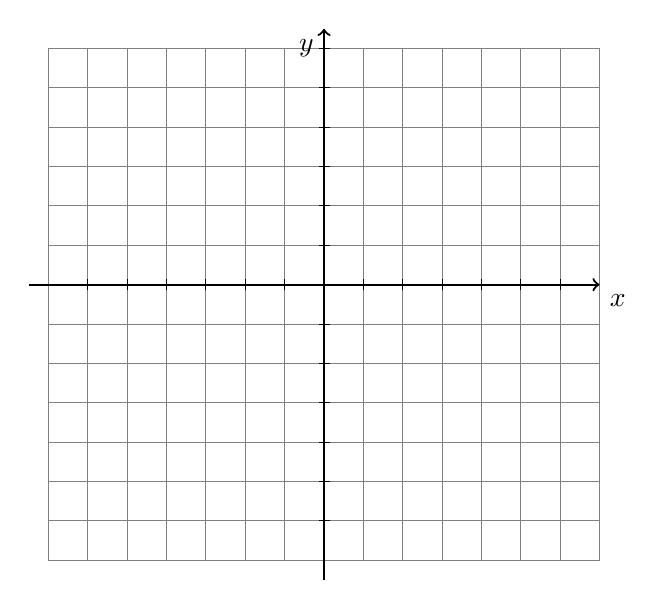
\begin{tikzpicture}[y=.5cm, x=0.5cm,font=\sffamily]
    %% ticks
    \draw[step = 1, gray] (-7,-7) grid (7,6);
    %% axis
    \draw[thick,->] (-7.5,0) -- coordinate (x axis mid) (7,0) node[anchor = north west] {$x$};
    \draw[thick,->] (0,-7.5) -- coordinate (y axis mid) (0,6.5) node[anchor = north east] {$y$};
    \foreach \y in {-6,-5,...,-1,1,2,...,6} {
      \draw (2pt, \y) -- (-2pt, \y);
    }
    \foreach \x in {-6,-5,...,-1,1,2,...,6} {
      \draw (\x,2pt) -- (\x,-2pt);
    }

\end{tikzpicture}


\vfill
\item Find a logarithmic function of the form $f(x)=b+\log_{a}(x+c)$ that has the vertical asymptote $x=-14$, passes through the point $(-13, 2)$ and crosses the $x$-axis at $x=\frac{-685}{49}$.
\vfill
\vfill
\vfill

\clearpage



\item Simplify the expression without using a calculator.
\begin{enumerate}

\item $\log_3(9)$\\

\item $\displaystyle \log_2(\frac{1}{16})$\\

\item $\log_{1/7}(49)$\\



\end{enumerate}







\item Simplify the expression without using a calculator.
\begin{enumerate}

\item $\displaystyle \log_4(4^{11})$\\

\item $\displaystyle 5^{\log_5(x+y)}$\\

\item $\log_{\pi}(1)$\\



\end{enumerate}






\item Write the logarithm as a sum or difference of logarithms and simplify as much as possible.  (Expand the logarithmic expression.)
\begin{enumerate}
\item $ \displaystyle \log_7\left(\frac{1}{7}mn^2\right)$ 
\vfill
\item $\displaystyle \log_5\left(\frac{p^5}{m\sqrt{n}}\right)$ 
\vfill

\item $\displaystyle \log\left(\frac{10}{\sqrt{a^2+b^2}}\right)$ 
\vfill

\item $\displaystyle \ln\left(\sqrt[5]{\frac{e^2}{c^2+5}}\right)$ 
\vfill


\end{enumerate}

\clearpage

\item Write the logarithmic expression as a single logarithm with coefficient 1, and simplify as much as possible.  (Condense the logarithmic expression.)


\begin{enumerate}
\item $\ln(y)+\ln(4)$\vfill
\item $\log_3(693)-\log_3(33)-\log_3(7)$\vfill
\item $3[\ln(x)-\ln(x+3)-\ln(x-3)]$\vfill
\item $\displaystyle 15\log(c)-\frac{1}{4}\log(d)-\frac{3}{4}\log(k)$\vfill
\end{enumerate}






\end{enumerate}


